\chapter{Sicurezza}

\section{Principi di sicurezza}
La sicurezza informatica pone le fondamenta in due principi fondamentali:
\begin{itemize}
    \item A.A.A.
    \begin{itemize}
        \item Authentication (autenticazione), capacità di un sistema di garantire che un utente possa essere identificato tramite informazioni in suo possesso
        \item Authorization (autorizzazione), indica che cosa può effettuare un determinato utente.
        \item Accounting (accreditamento), la procedura con cui si assegnano determinate operazioni effettuate a un account
    \end{itemize}
    \item C.I.A.
    \begin{itemize}
        \item Confidentiality (confidenzialità), un messaggio si può definire confidenziale se può essere letto solo dal destinatario predesignato
        \item Integrity (integrità), un messaggio può essere considerato integro se il destinatario è certo del suo mittente
        \item Availability (disponibilità), la disponibilità è la capacità di un sistema di rispondere a determinate richieste
    \end{itemize}
    essendo concetti indipendenti tra di loro, per poter garantire la sicurezza del sistema essi dovranno essere presenti tutti e tre contemporaneamente
\end{itemize}
Una proprietà non presente in CIA (perché non rappresenta la sicurezza di un sistema ma un modo di eludere la proprietà di accounting) è \textbf{l'anonimato} online.
Navigando online non si è anonimi, in quanto si è soggetti a profilazione dagli ISP, cookie traccianti ecc.
\section{Riassunto di reti}
\subsection{Protocolo di rete}
Per identificare un server, o più in generale un dispositivo sulla rete, si una il protocollo IP (Internet Protocol), il più utilizzato è la versione 4, che prevede quattro quartine di 8 byte l'una per un totale di 32 bit. Il server per poter rispondere a una nostra richiesta in questo caso dovrà necessariamente conoscere il nostro indirizzo IP, ciò porta a non avere anonimato sulla rete.
\subsection{IP Spoofing}
Gli indirizzi IP per costruzione non sono protetti da una forma di integrità, questo significa che chiunque può cambiare il proprio indirizzo IP sorgente per fingersi qualcun altro.
\subsection{Routing}
Un pacchetto per essere consegnato al destinatario verrà fatto passare attraverso un infrastruttura di router i quali per definizione sono Man in the Middle, portandoci quindi a doverci fidare della rete se facciamo passare i dati in chiaro.
\subsection{TCP (Transmission Control Protocol)}
Il protocollo più utilizzato per stabilire una connessione con un server è il TCP, al livello superiore questo protocollo identifica i servizi oltre all'indirizzo IP anche mediante una porta. Alcune porte sono difinite dallo standard è si utilizzano per determinati servizi:
\begin{itemize}
    \item 22 - SSH
    \item 25 - SMTP (mail in uscita)
    \item 100 - POP (mail in entrata)
    \item 80 - HTTP
    \item 443 - HTTPS
\end{itemize}

\subsubsection{Attacco a TCP: Syn flooding}
\begin{wrapfigure}{r}{0.5\textwidth}
    \begin{center}
        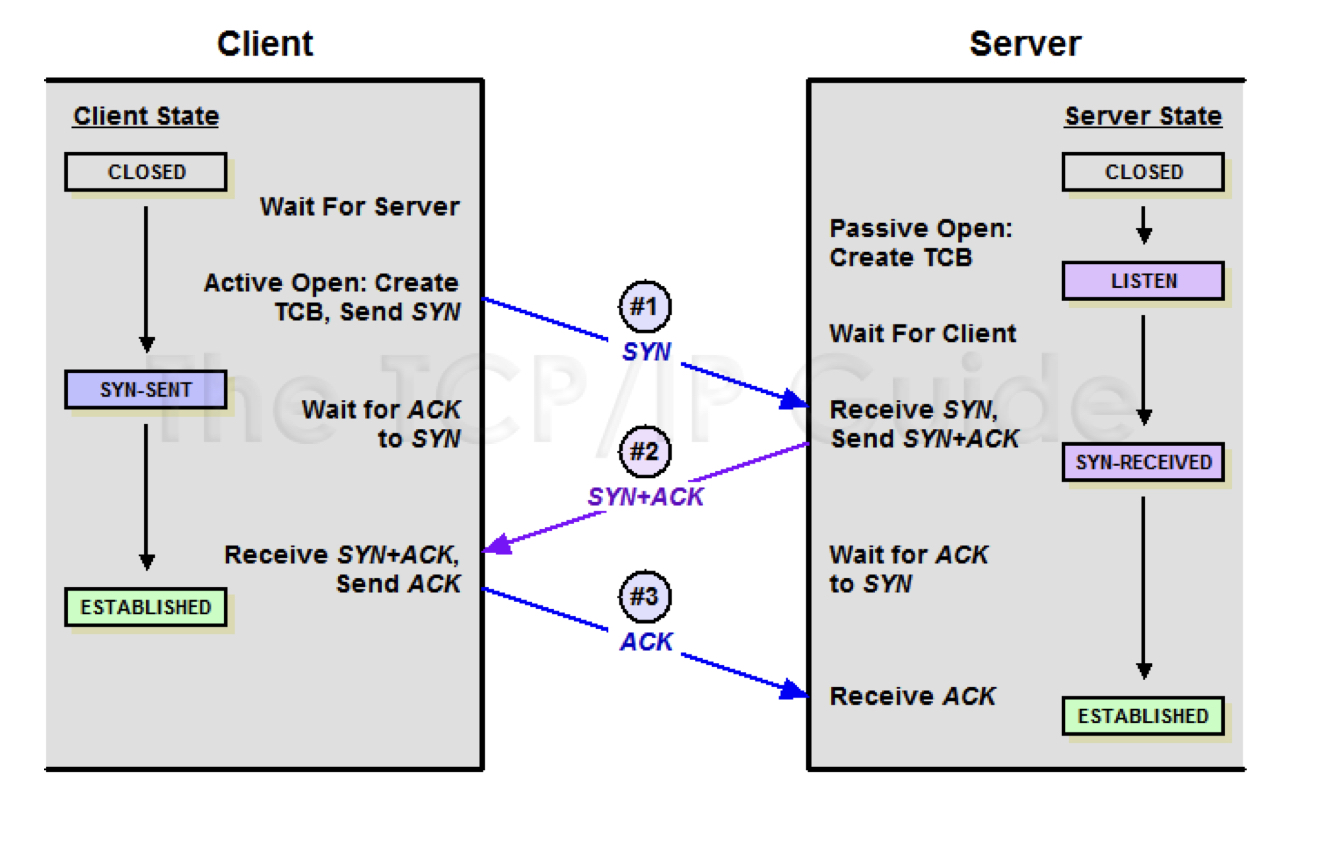
\includegraphics[width=0.5\textwidth]{res/3way-handshake.png}
    \end{center}
\end{wrapfigure}
Il protocollo TCP al contrario di altri protocolli dello stesso livello come UDP (User Datagram Protocol) è un protocollo orientato alla connessione, per effettuare ciò TCP in via un pacchetto con una segnalazione speciale chiamata \textbf{SYN}, inviato questo pacchetto si aspetterà un altro pacchetto con una segnalazione di tipo \textbf{SYN-ACK}, e infine una volta arrivatogli risponderà con un pacchetto di segnalazione di tipo \textbf{ACK}, questo modo di stringere la connessione prende il nome di \textbf{3-Way Handshake}.

Sfruttando questa cosa a nostro vantaggio, cosa succede se non si invia mai l'ACK finale e il server può accettare massimo $n$ chiamate? \\
Si otterrà un attacco di tipo Denial of Service (DoS) dopo $n$ chiamate rendendo impossibilitato il server a rispondere alle varie connessioni.

\subsection{DNS (Domain Name Service)}
Il mondo dei servizi online per questione di praticità non ragione in termini di indirizzi, troppo complessi da ricordare e facilmente soggetti a errori di scrittura, per questo motivo è esiste un registro online distribuito chiamato \textbf{DNS}

\subsubsection{Attacco a DNS: Typosquatting}
Cosa succede se comprassimo il dominio gmail.it?
Tutte le persone che sbaglieranno a scrivere l'indirizzo email da gmail.com a gmail.it invieranno le loro email al nostro server, questo ci farebbe entrare in possesso di email private senza nemmeno dover effettuare social engineering.

\subsection{Sniffing}
Lo sniffing è una forma di Eavesdropping e può essere messo in atto da chiunque lungo tutto il percorso verso la destinazione del pacchetto. Lo sniffing si può effettuare in tutti i protocolli già citati, e.g. sniffing DNS che ci permette di entrare a conoscenza di tutti i siti visitati, sniffing TCP che ci rivela ciò che si sta chiedendo al server etc.

\section{Anonimizzazione}

\subsection{Anonymous remailer}
Prendendo in considerazione il caso più semplice, cioè l'invio di email anonime.
Un anonymous remailer è un server che ricevuta un'email (con le informazione sul destinatario) prende questa email e la inoltra al destinatario rimuovendo le informazioni del mittente.
Un esempio di molto simile è ciò che sta alla base delle VPN.
Un anonynous remailer è un esempio di proxy. Il problema dei proxy però è che hanno informazioni sul nostro traffico, ciò lo rende facilemnte utilizzabile come eavesdropper.

\subsection{Routing a cipolla}
Per anonimizzare completamente il traffico è possibile usare il cosiddetto Routing "a Cipolla" (Onion Routing).
Il software più famoso che rende possibile ciò è Tor (The Onion Routing) che utilizza questi concetti per anonimizzare il traffico.

\begin{figure}[h!]
    \centering
    \begin{subfigure}{.5\textwidth}
        \centering
        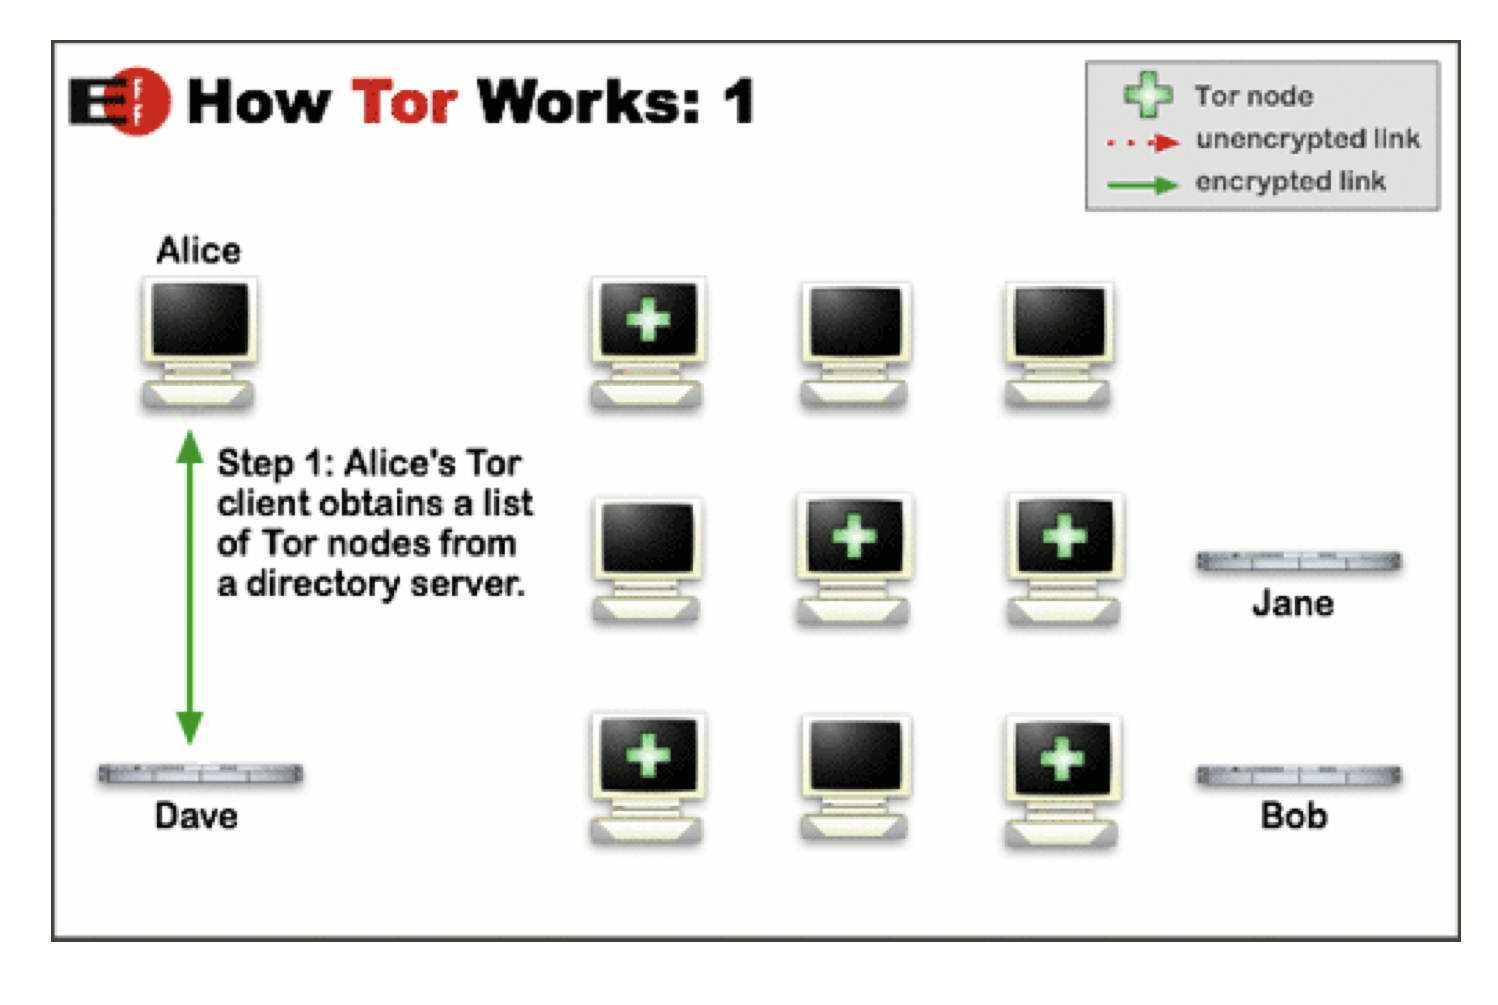
\includegraphics[width=1\linewidth]{res/tor1.png}
    \end{subfigure}%
    \begin{subfigure}{.5\textwidth}
        \centering
        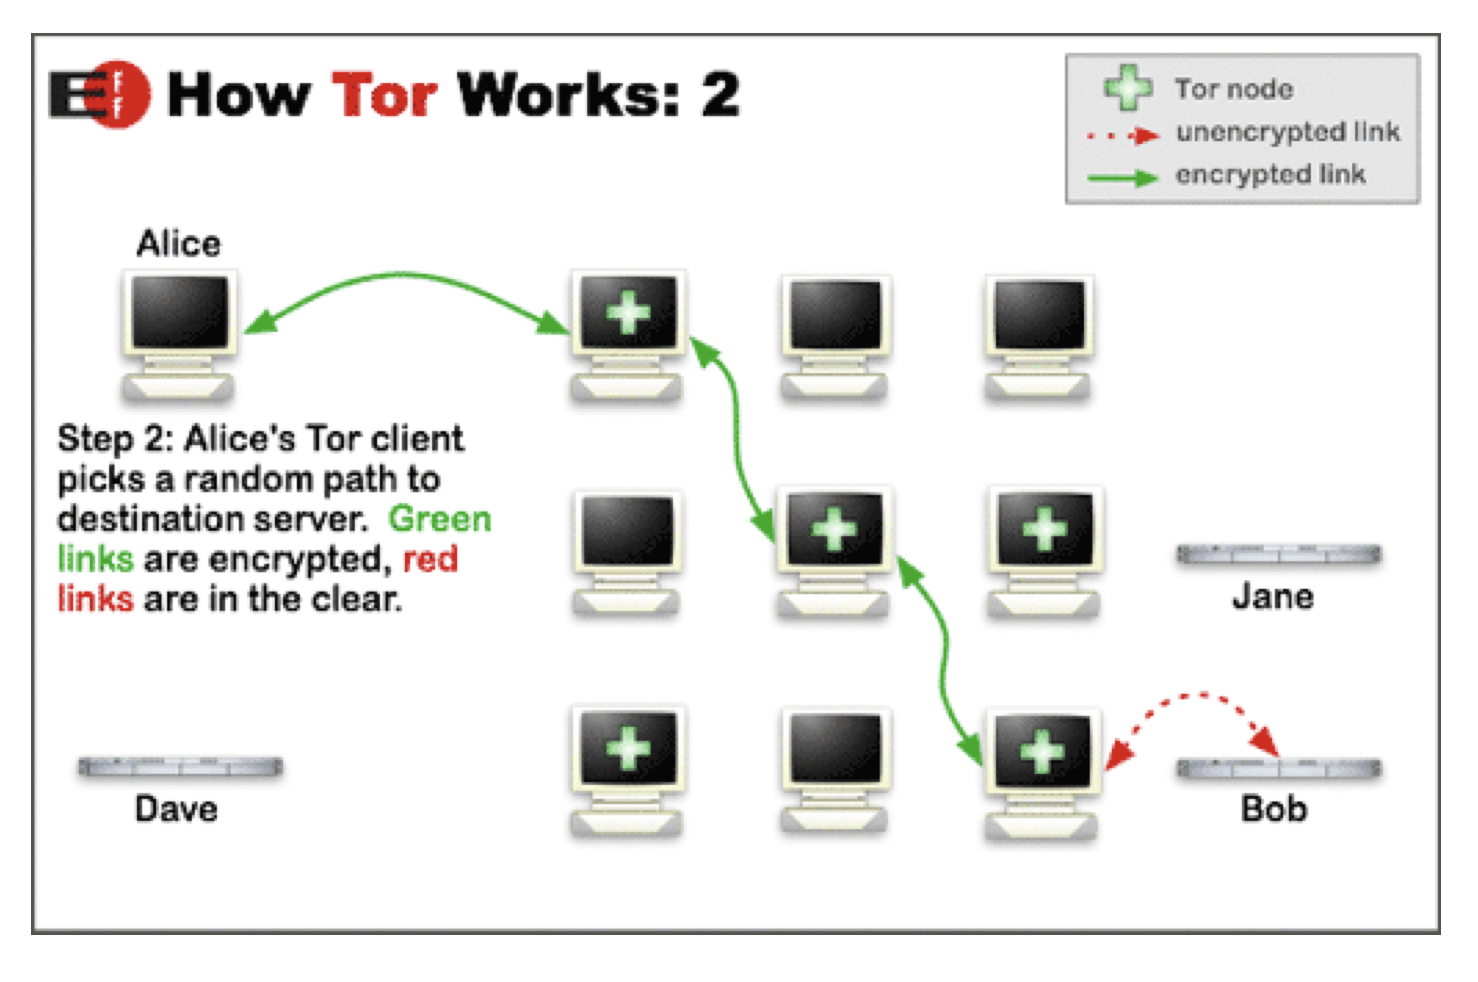
\includegraphics[width=1\linewidth]{res/tor2.png}
    \end{subfigure}
    \begin{subfigure}{.5\textwidth}
        \centering
        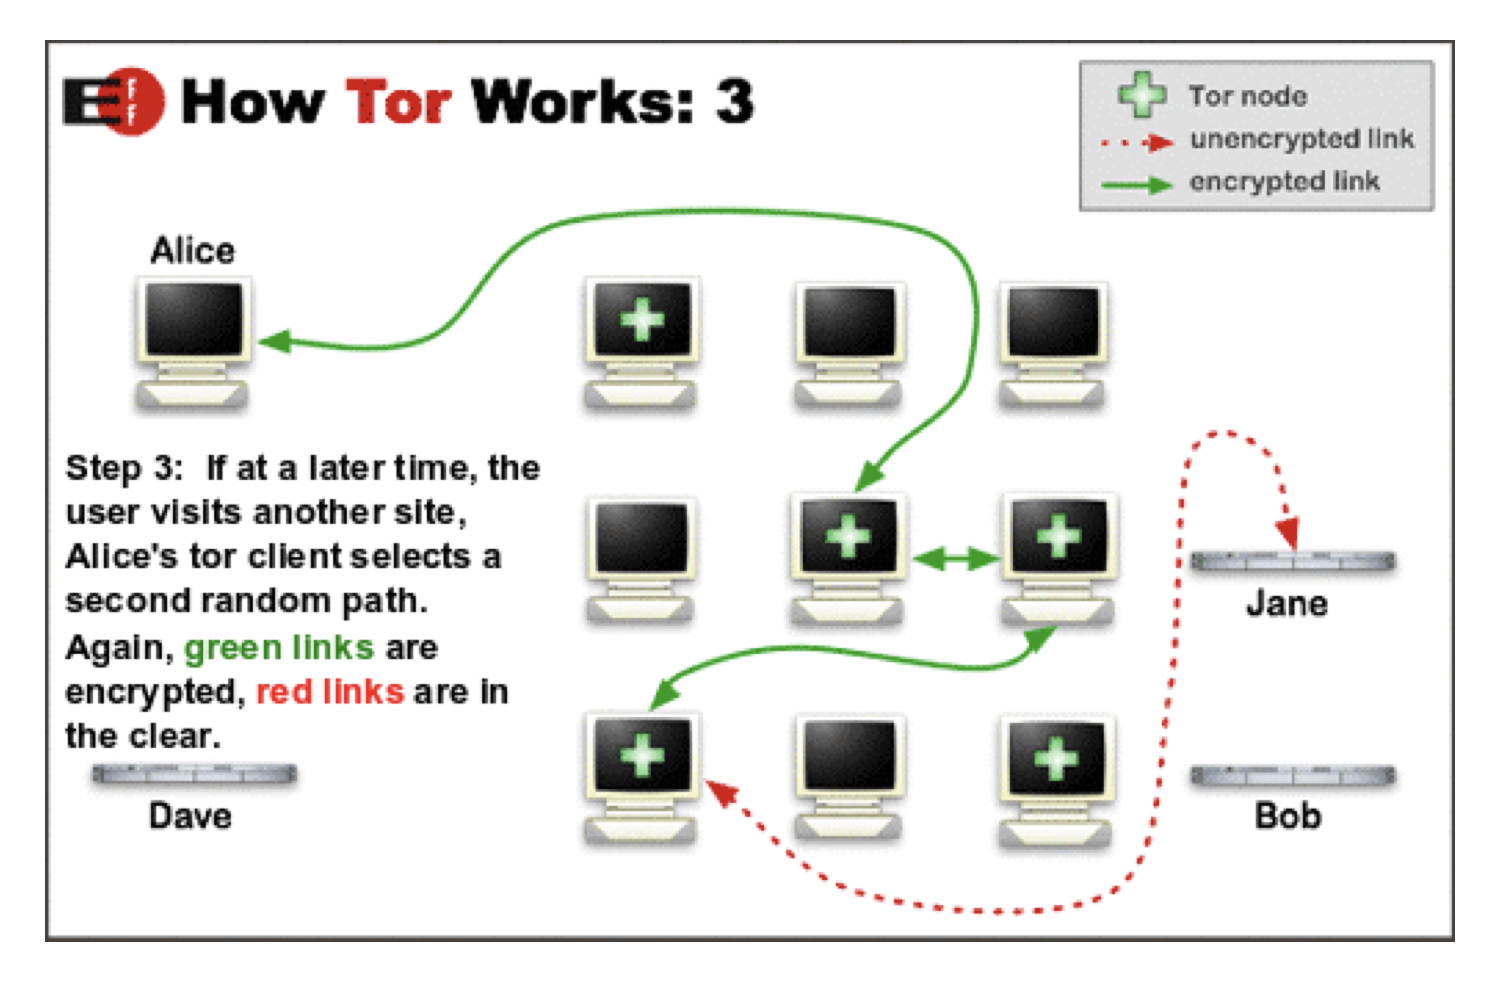
\includegraphics[width=1\linewidth]{res/tor3.png}
    \end{subfigure}
\end{figure}
Tor è un protocollo studiato per mantenere l'anonimato sulla rete basandosi sul routing a cipolla.
L' \textbf{\textit{Onion Routing}} consiste nell'incapsulare il pacchetto in vari strati, da qui il nome routing a cipolla, il client al momento dell'invio del pacchetto sceglierà il percorso da fargli fare, sempre casuale, e cripterà ogni strato in modo tale che sia eliminabile da un solo nodo del percorso, così facendo il pacchetto verrà inviato al primo nodo che lo "pelerà" dal primo strato e lo spedirà al secondo nodo che farà lo stesso e così via una volta arrivato all'ultimo nodo il pacchetto sarà decifrato totalmente e verrà inviato in chiaro al server destinatario.
Ognuno dei nodi dal secondo all'ultimo che utilizzeremo sarà a conoscenza solo del nodo precedente e successivo, questo ci garantisce l'anonimità della connessione, solo il primo nodo sarà a conoscenza del mittente ma come gli altri non sarà a conoscenza del contenuto del messaggio e del destinatario finale che al contrario sarà conosciuto solo dall'ultimo nodo (exit node).
\begin{figure}[h!]
    \centering
    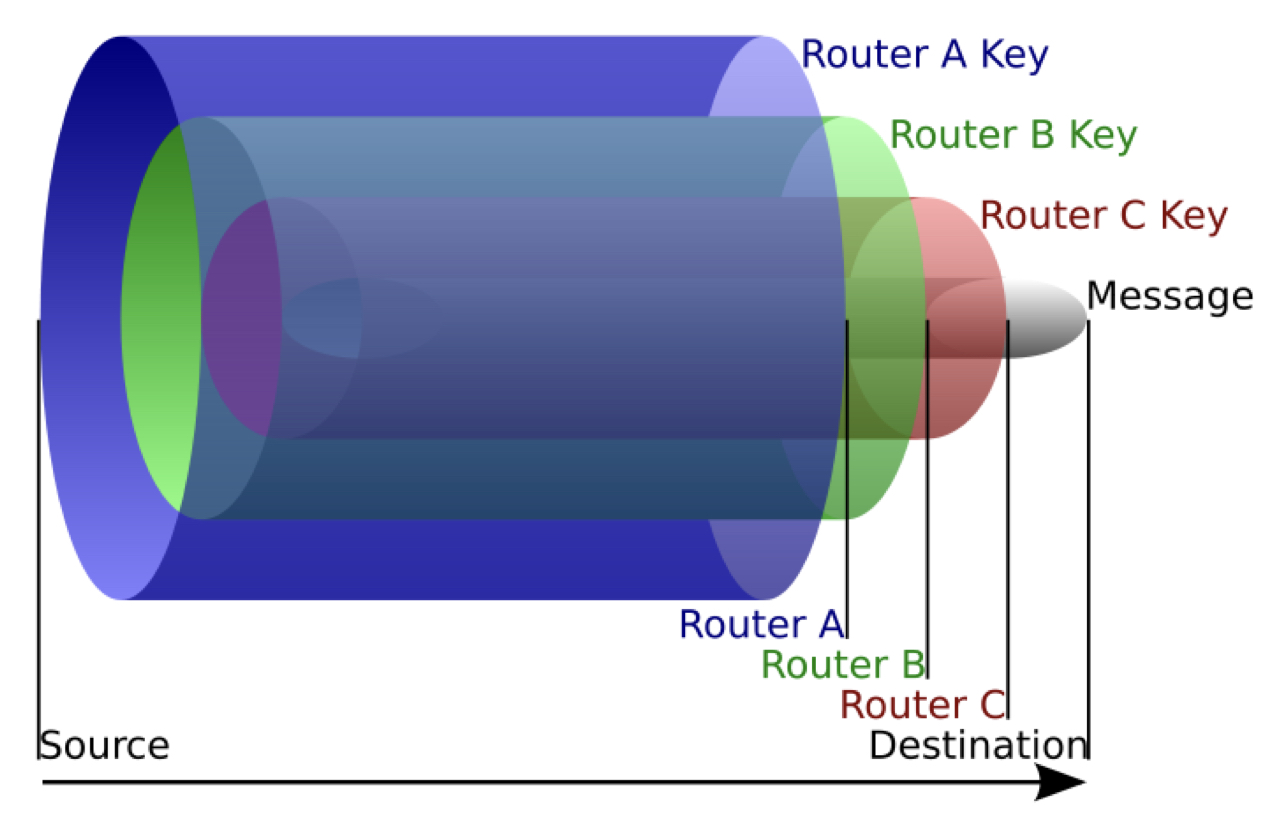
\includegraphics[width=.8\linewidth]{res/tor-encryption.png}
    \caption{}
\end{figure}
Tor viene quindi soprannominata rete overlay. Una rete chiusa al quale all'interno vengono distribuiti dati in forma anonima.
Garantendo l'anonimato al suo interno è spesso utilizzata per fornire dei servizi illegali.
Un comportamento molto presente sui servizi onion è la compravendita di Dataleak (informazioni private di aziende, persone o oggetti).
Due dei dataleak più importanti sono quelli di tipo Fullz e Password:
\begin{itemize}
    \item Fullz: collezione di infoermazioni personale contenenti almeno il minimo indispensabile per creare conti correnti e/o pagare con carte di credito, utili per perpetrare truffe molto più facilmente:
    \begin{itemize}
        \item Nome e Cognome
        \item Data di nascita
        \item Codice Fiscale
        \item Indirizzo di residenza
        \item Numero di telefono
    \end{itemize}
    \item Password: sono i leak di informazioni più comuni in cui viene messa online una lista di account e password di qualche servizio pronte per essere acquistate da qualcuno.
\end{itemize}
Anche se Tor è molto sicuro purtroppo è afflitto anch'esso da falle:
\begin{itemize}
    \item Geolocalizzazione: se attiva porterebbe a rivelare l'ip dell'utilizzatore di un servizio anche con Tor;
    \item DNS: un altra falla è la possibile richiesta DNS all'esterno che porterebbe l'attaccante a sapere il servizio da noi visitato;
\end{itemize}
Le informazioni rivelate non devono per forza essere direttamente collegate a vostre richieste ma possono essere informazioni "laterali" (Side Channel), come la dimensione in cui siamo abituati a tenere la finestra del browser la percentuale di luminosità dello schermo ecc. che se inviate al server remoto porterebbe lo stesso a una profilazione.
Per sopperire a queste problematiche la chiave è rilasciare non più informazioni di quelle strettamente necessarie.